\chapter{Computational Speed up of RL-MPC}
\label{chapter:speed-up}

This chapter aims to provide an overview of the application of making the best-performing RL-MPC (RL-MPC 5) algorithm more computationally efficient. While the controller has demonstrated a marginal increase in computational time compared to nominal MPC at lower prediction horizons, incorporating a neural network as a cost function in larger and more intricate systems may introduce excessive delays and hinder performance. Two experiments were conducted to achieve speedup, and the resulting performance and computational time were investigated. Given that the longer computation time is caused by the inclusion of the value function in the formulation of the MPC algorithm, it is logical to focus on optimising this aspect to improve speed. Three approaches were devised to accelerate the algorithm, with the initial one involving training a less intricate surrogate value function instead of employing the full complex neural network for the terminal cost function. The procedure above has previously been performed, and the resulting outcomes were documented in \autoref{chapter:deterministic_RL_MPC}. ${V}_{\phi_4}$can be regarded as a surrogate value function for ${V}_{\phi_1}$. The surrogate value function exhibited greater stability and computational efficiency than the full order model. Consequently, it was employed in all subsequent experiments due to its stability. The following experiments were designed to accelerate the algorithm by implementing further simplifications to the neural network. It is important to note that the following experiments were performed on the deterministic environment with zero parametric uncertainty.

\section{Reducing Neurons and Hidden Layers}
A simple yet effective approach was to reduce the size of the neural network representing the value function. The policy on which the value function was trained remained fixed. All neural networks were trained with the same hyperparameters outlined in \autoref{section:trained-vf}. An investigation was conducted on multiple network architects. The initial architecture, on which previous results have been established and will be considered the baseline performance, comprised a deep neural network with two hidden layers, each containing 128 neurons. It was decided to have three deep and three shallow neural networks to create the smaller neural networks. There are 128, 64 and 32 neurons in each hidden layer for the deep and shallow networks. Doing this effectively generates neural networks that become simpler as the number of neurons and hidden layers decreases, making it possible to examine the impact of the complexity of the neural network on the RL-MPC’s performance and computational time. It is important to note that both hidden layers use the same number of neurons for the deep neural networks.

\begin{figure}[H]
	\centering
	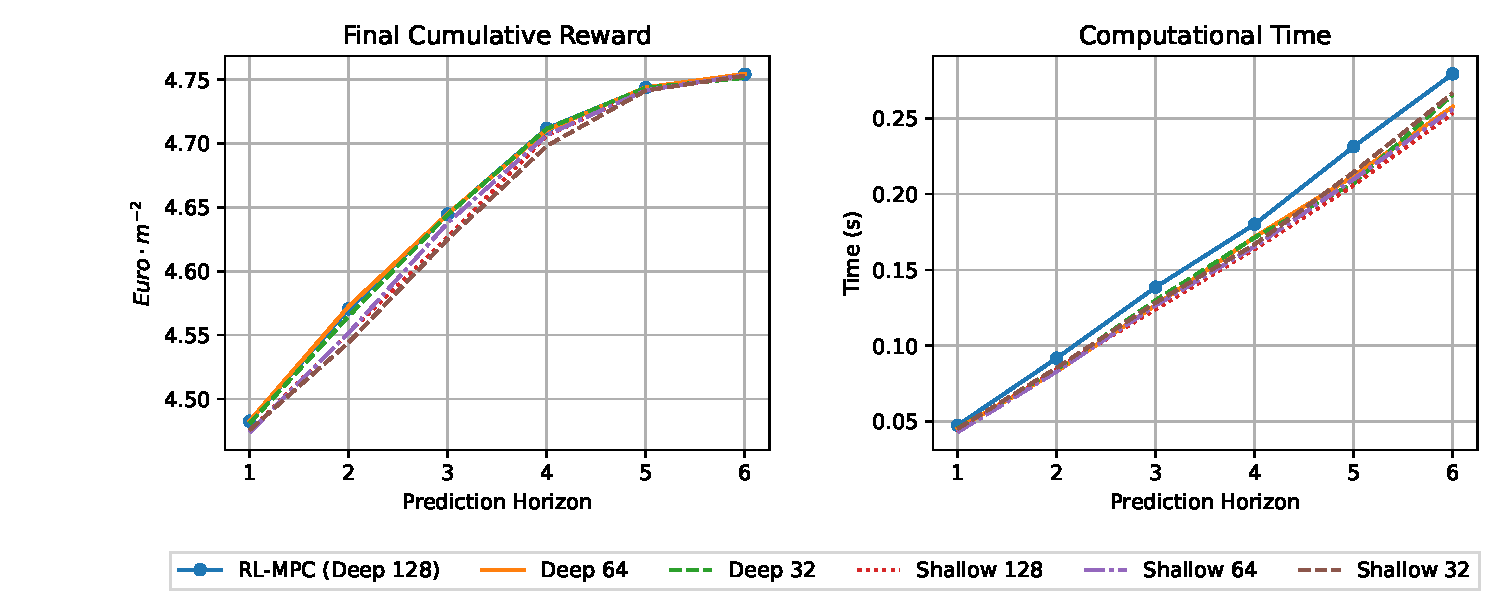
\includegraphics[width=\textwidth]{figures/speed_up_neurons.pdf}
	\caption{Fast RL-MPC with reduced neurons}
	\label{fig:neurons-speedup}
\end{figure}

The performance gains, in terms of final cumulative reward, and the computational time of the RL-MPC controller with different neural network architectures vs prediction horizon are shown in \autoref{fig:neurons-speedup}. It is evident that the simpler models reduce computational time but at the expense of decreased performance. To be more precise, it appears that all simpler neural networks have comparable computational times. However, shallow neural networks have a much more pronounced negative effect on performance than deep neural networks, which have a minimal impact on performance.

\begin{figure}[H]
	\centering
	\resizebox{.7\textwidth}{!}{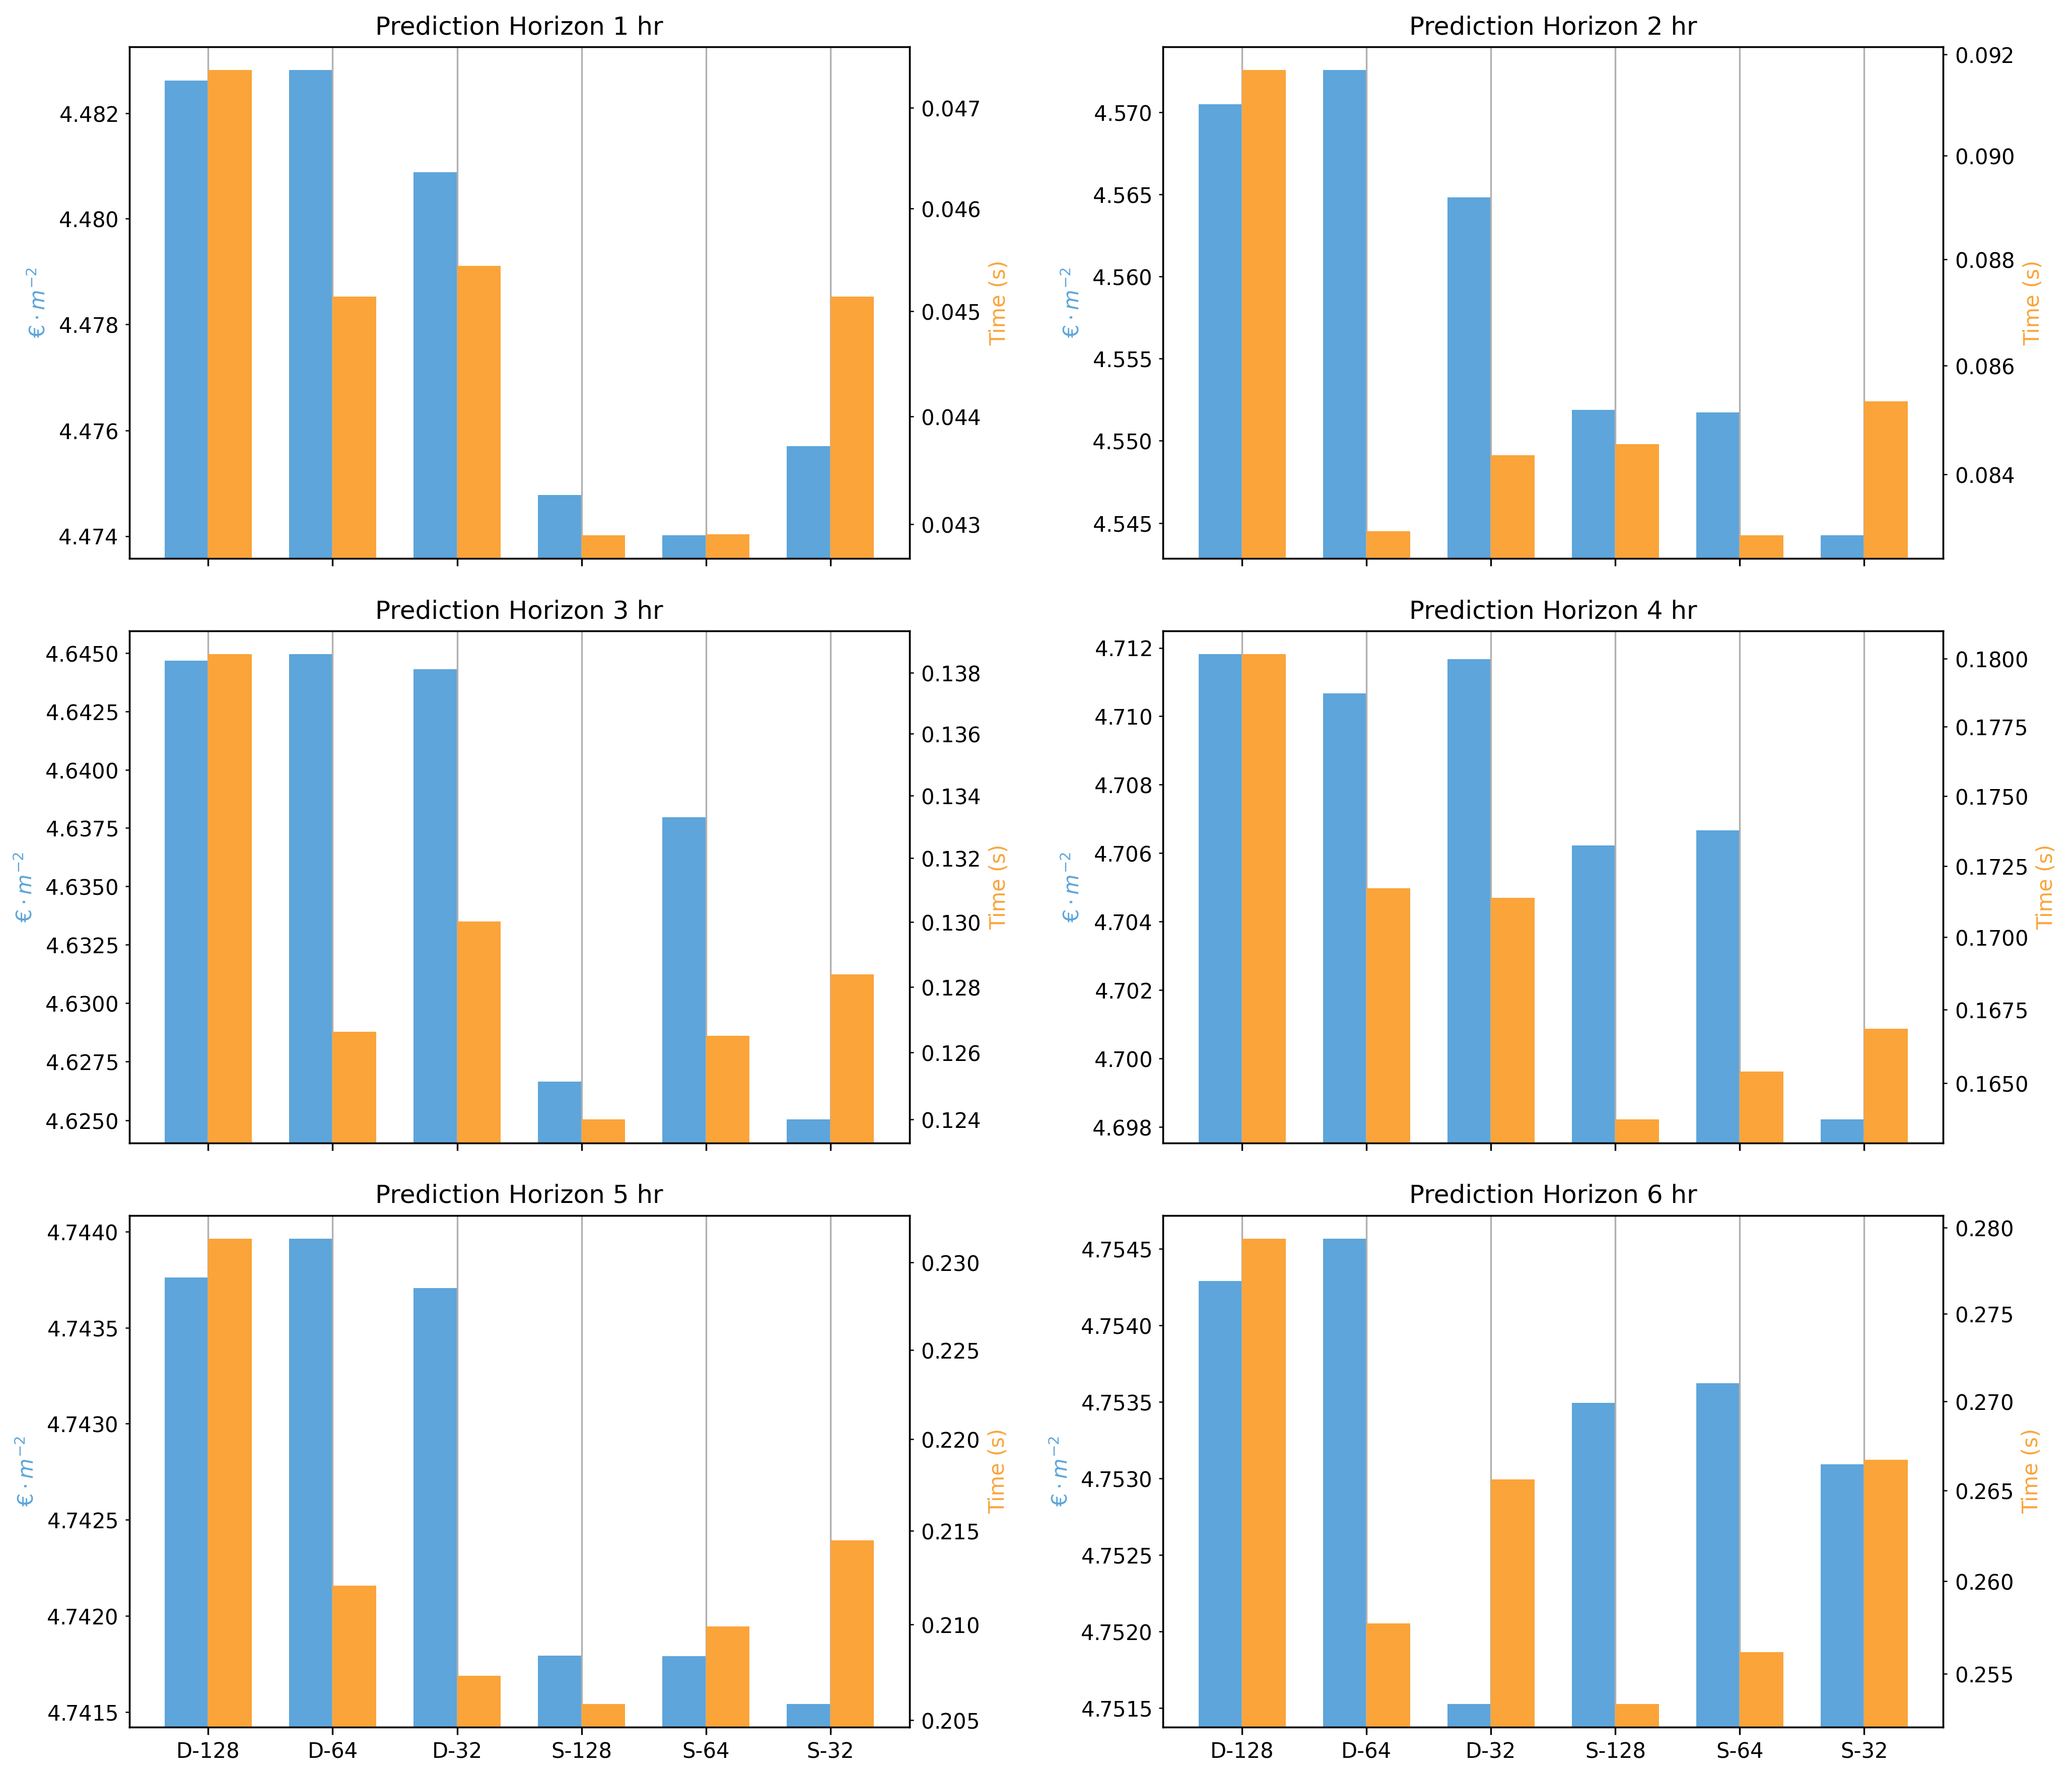
\includegraphics{figures/speed_up_neurons_bar_graph.png}}
	\caption{RL-MPC with reduced neural network complexity for its terminal cost function, where D-128 would stand for ''Deep neural network of 128 Neurons per hidden layer''.}
	\label{fig:neurons-speedup-bar-graph}
\end{figure}

\autoref{fig:neurons-speedup-bar-graph} displays a more in-depth analysis of the performance gains and computational times of the tested neural networks vs prediction horizon. From \autoref{fig:neurons-speedup-bar-graph}, There is no observable correlation between the complexity of the neural network and the improvements in performance and computational time. Contrary to expectations, decreasing complexity does not necessarily result in a decrease in performance and time. However, it suggests that a simpler network can result in lower computational times, albeit at the cost of performance. Furthermore, \autoref{fig:neurons-speedup-bar-graph} suggests that shallow networks offer less benefit due to their substantial decrease in performance compared to the simpler deep neural networks. The most effective neural network architecture appears to be a deep neural network with 64 neurons per hidden layer. This architecture achieves a very similar performance to the original deep neural network with 128 neurons per layer but with a noticeable reduction in computational time for all prediction horizons. This can be seen in \autoref{fig:neurons-speedup} and \autoref{fig:neurons-speedup-bar-graph}. Thus, these findings indicate that, while reducing network complexity can speed up the algorithm with minimal to no performance degradation, comprehensive testing of the neural network architecture is necessary to achieve this.


\section{Taylor Approximation}

Perhaps a more intuitive approach would be to use a Taylor expansion around a point to approximate the neural network locally to achieve speedup. The Taylor expansion provides a first-order (linear approximation) or a second-order (quadratic approximation) of the neural network’s outputs concerning its inputs. Calculating the Jacobian of a neural network, which is required for the first-order Taylor approximation, is generally considered straightforward. However, analytically determining the Hessian of a neural network, used in the second-order Taylor approximation, is considerably more difficult and computationally intensive. Nevertheless, employing a second-order Taylor approximation would result in more precise approximations around the chosen point, potentially leading to better value function approximations and, therefore, an increase in performance. Fortunately, since the structure of the neural network does not change over the control period, the Jacobian and Hessian only need to be analytically calculated once.

The Taylor expansion of the neural network was accomplished using CasADi and L4CasADi. The first- and second-order Taylor expansions were conducted around the terminal point, which is determined by the initial guess ($\tilde{\mathbf{x}}_{k|k},\tilde{\mathbf{u}}_{k|k}$), for every time step. The performance and computational time of these approximations were compared to the original RL-MPC 5 implementation.

\begin{figure}[H]
	\centering
	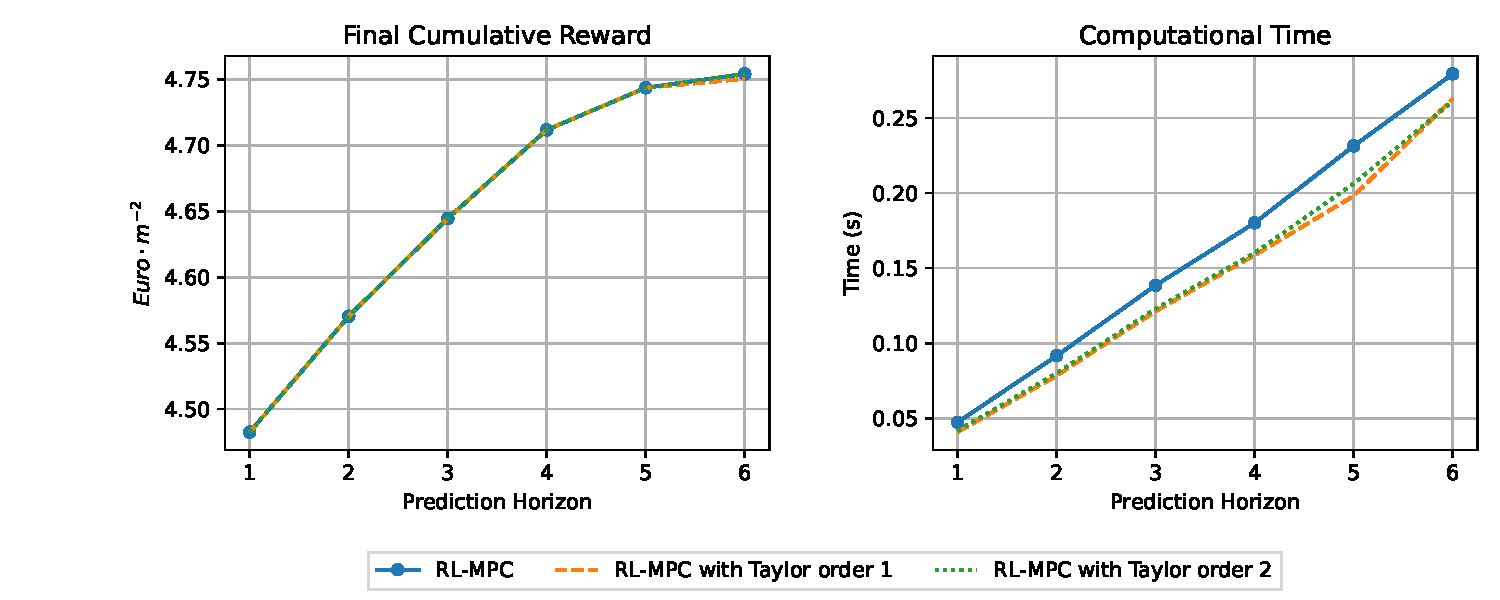
\includegraphics[width=\textwidth]{figures/taylor_speed_up.pdf}
	\caption{Fast RL-MPC with Taylor approximation}
	\label{fig:taylor-speedup}
\end{figure}

The impact of a linear and quadratic approximation of the neural network around the terminal guess is illustrated in \autoref{fig:taylor-speedup}. Locally approximating the neural network has evident advantages, as both first- and second-order approximations result in a substantial reduction in computational time without any noticeable decline in performance. It appears that a second-order approximation is unnecessary, and a first-order approximation may be preferable due to its lower computational time without sacrificing performance.


\section{Combined}
The following study investigated the combined effects of the two speedup techniques on the RL-MPC algorithm. The experiment includes combining the best results from the previous two experiments.


\begin{figure}[H]
	\centering
	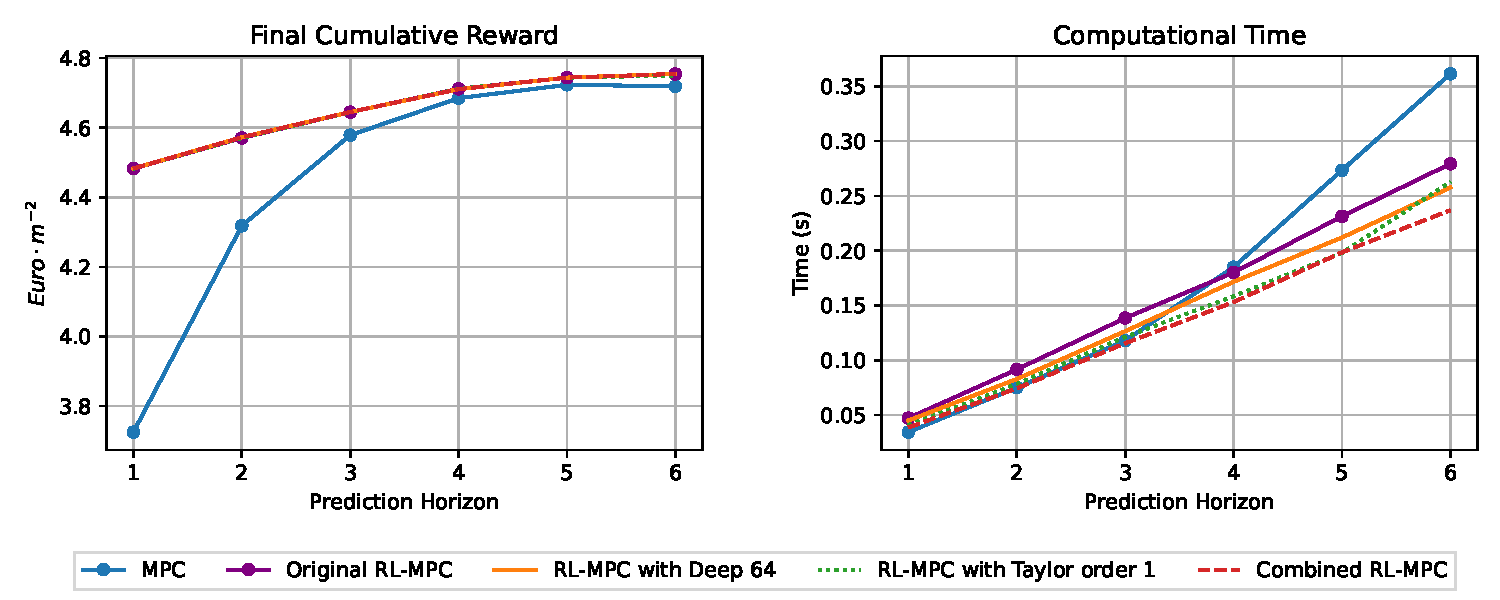
\includegraphics[width=\textwidth]{figures/final_speed_up.pdf}
	\caption{Fast RL-MPC}
	\label{fig:final-speedup}
\end{figure}

The results of using a deep neural network with 64 neurons per hidden layer and a first-order Taylor approximation around the terminal guess are presented in \autoref{fig:final-speedup}. These findings are compared to the individual speedup techniques used, the original RL-MPC and the nominal MPC. Similar to previous results, \autoref{fig:neurons-speedup} and \autoref{fig:taylor-speedup}, the combined techniques have zero or little impact on the performance. Although using a first-order Taylor expansion reduces computational time more than a smaller deep neural network, combining both methods further decreases computational time. The final reduction is significant enough that the computational cost becomes equivalent to or less than that of MPC, even at shorter prediction horizons of 1, 2 and 3 hours. These results are significant because they demonstrate the successful implementation of methods that achieve speedup without compromising performance. These findings could have even greater implications for more complex (greenhouse) systems, where achieving real-time control or minimising delay is crucial for system performance.


\section{Discussion and Conclusion}
Based on the findings of this chapter, it is evident that a speedup of the RL-MPC can be achieved. This speedup can be achieved by focusing on strategic adjustments to the neural network used in the terminal cost function. The experiments detailed in this chapter aimed to reduce computational time with little to no performance impact.\\
Initially, efforts focused on making the neural network smaller by reducing neurons and hidden layers. This approach showed that changing the number of neurons and hidden layers has a noticeable impact on performance and computational time. However, there was no discernible relationship between simpler models and faster computational time or performance improvements. Nevertheless, the results indicated that shallow neural networks generally have a higher trade-off between performance improvements and computational time than deep neural networks. It was found that a deep neural network with 64 neurons per hidden layer reduced computational time with no performance losses compared to the original deep neural network with 128 neurons per hidden layer. Thus, it is necessary to search the design space thoroughly to achieve the desirable reduction in computational time when designing the RL-MPC algorithm for other systems. \\
Moreover, applying Taylor approximations, both linear and quadratic, around the terminal guess provided further insights into reducing computational time. For both linear and quadratic approximations, the speedup in computational time was noticeable while having no impact on the performance, particularly the first-order approximation. In addition, the Jacobian of a neural network is substantially easier to compute than the Hessian. Consequently, opting for a linear approximation may be a more attractive option.\\
Combining these two approaches yielded the most promising results. A smaller deep neural network of 64 neurons per hidden layer with a first-order Taylor approximation achieved computational speeds comparable to or faster than the nominal MPC for every prediction horizon tested. Not only was the amount of time required for computation decreased, but there was also no noticeable decline in performance. \\
In conclusion, these findings underscore the feasibility of enhancing RL-MPC’s computational efficiency by thoughtful adjustments in neural network complexity and approximation techniques. Such optimisations are crucial for scaling RL-MPC applications to more intricate systems, potentially facilitating real-time control and minimising delays, consequently enhancing overall system performance. Future research may explore further refinements to the structure of the cost function, potentially using alternative, more intuitive non-linear function approximators instead of neural networks.

